%&pdflatex
%\vspace{-0.3458cm}
\section{Perceptual Reasoning with the Containment Graph}
\label{sec:reasoning}
%\vspace{-0.258cm}
The successful manual sequence of transforms in Figure~\ref{fig:tiger:sequence} is one among numerous many: Initially and after applying a transform sequence, there are typically a number of transforms which are applicable next. This leads to an exponential search space which quickly becomes impractical. Two key observations reduce the search space to a manageable size: {\em (i)} not all transform sequences are plausible, and {\em (ii)} there is a significant duplication in that two distinct transform sequences can result in the same fragment. We propose the idea of a {\em containment graph} to implement both. 

First, the state of an image at any point in the course of applying transforms is represented by a node, and the set of applicable transforms at each stage are represented by links. Observe that two transform sequences applied to two distinct fragments can lead to the same state, especially when the two fragments are adjacent or the same. Figure~\ref{fig:containment:graph}b. The containment graph is constructed in a breath first manner and effectively represents inherent grouping ambiguity by representing each grouping hypothesis as a node. The containment graph nodes are our proposed mid-level representation to be used by high level processes.

\begin{figure*}[ht]
%\vspace{-0.61cm}
\hbox{
\vbox{
\hbox{
{\footnotesize\textit{(a)}}
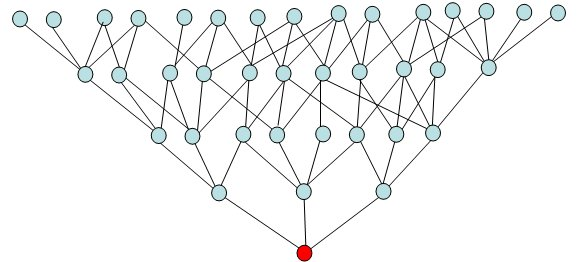
\includegraphics[width=0.25\textwidth]{figs/hypothesis-tree.jpg}
}
\hbox{
\hspace{-0.25cm}{\footnotesize\textit{(c)}}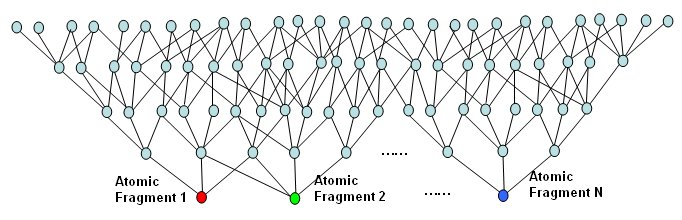
\includegraphics[width=0.4\textwidth]{figs/merged-hypothesis-trees.jpg}
}
}
\hspace{-0.85cm}{\footnotesize\textit{(b)}} \hspace{0.1cm} \includegraphics[width=0.57\textwidth]{figs/elephant.pdf}
}
%\footnotesize\textit{(f)}}  \includegraphics[height=0.1851\textwidth]{figs/containment_graph.pdf}
 %{\footnotesize\textit{(c)}}  \includegraphics[height=0.0851\textwidth]{figs/ambiguous-grouping-org.png}
%{\footnotesize\textit{(b)}}  \includegraphics[height=0.0851\textwidth]{figs/ambiguous-grouping-1.png}
%{\footnotesize\textit{(c)}}  \includegraphics[height=0.0851\textwidth]{figs/ambiguous-grouping-2.png}
%\vspace{-0.32cm}
  \caption{\FigureFont (a) The graph of grouping possibilities involving
a single fragment. (b) An example graph for a fragment of an elephant. (c) The
union of  graphs  from all fragments is the   {\bf containment graph}.}
  \label{fig:containment:graph}
  %\vspace{-0.653cm}
\end{figure*}



Second, just as it is unwise to commit to a single grouping option at each grouping stage, it is equally unwise to keep all the options indiscriminately
against mounting evidence. The application of each transform sequence represents an ``investment based on faith'' since raw, proximal data is being manipulated to generate a possibly more structured and regular representation, \eg,
contour completion across a gap may close a shape.
The likelihood defined in Equation~\ref{eq:path_like} is therefore capped
at a minimum value to limit the exploration of highly unlikely transformation sequences. This leads to numerous terminal nodes in the containment graph.  
% \begin{figure}[!h]
%    \begin{center}
% %  {\footnotesize\textit{(b)}} 
% \includegraphics[height=0.11\textwidth]{figs/mushrooming.png}
% %\vspace{-0.35cm}  \end{center}
%   \caption{The number of perceptual fragment mushrooms out as compared to the number of atomic fragments, but surprising keeping track of the combinatorics via the containment graph  is not impractical.
% }
% \label{fig:mushroom}
% \end{figure}


\begin{figure}[h]
  %\vspace{-0.15cm}
a) 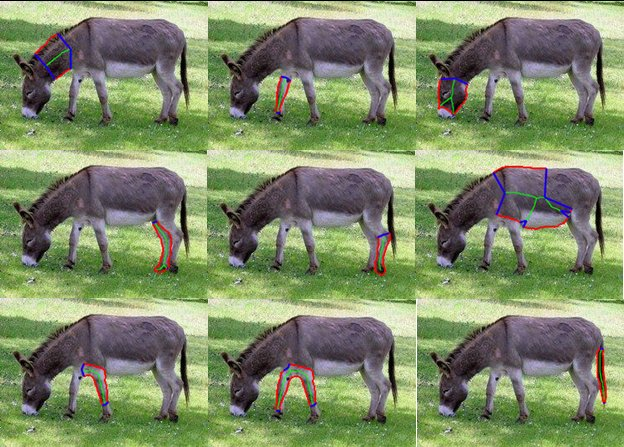
\includegraphics[width=0.43\linewidth]{figs/donkey-fragments-good.jpg}
b)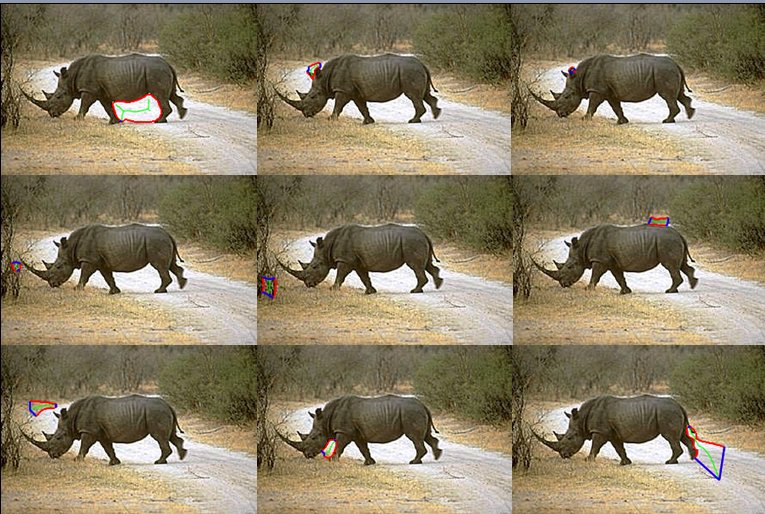
\includegraphics[width=0.43\linewidth]{figs/rhino-fragments-background.jpg}
%b)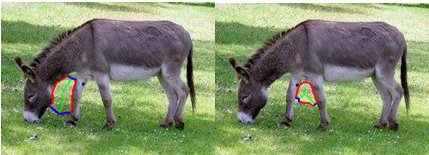
\includegraphics[width=0.45\linewidth]{figs/donkey-fragments-background.jpg}
%d) 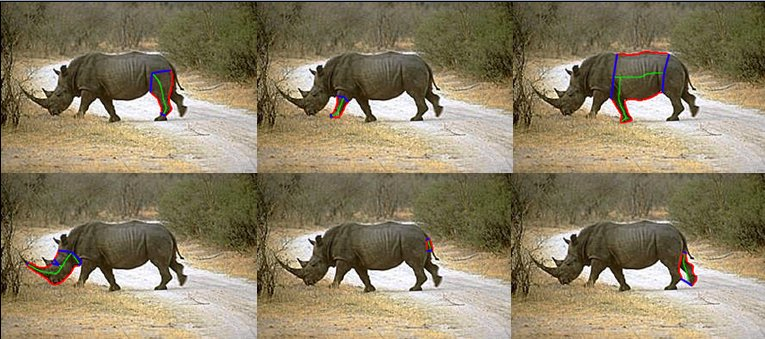
\includegraphics[width=0.48\linewidth]{figs/rhino-fragments-good.jpg}
%\vspace{-0.58cm}  
\caption{Selection of nodes from the containment graph: 
a) donkey fragments b) rhino fragments }
  \label{fig:donkey:fragments}
    %\vspace{-0.3cm}
\end{figure}

The value of using the containment graph can be measured by probing the total number of nodes explored with and without a containment graph. We expect that as the number of contour fragments increases so does the relative value of the containment graph. Figure~\ref{fig:graph_with_without} shows the relative number of nodes explored for a coarse scale version of the Weizmann Segmentation Dataset~\cite{Alpert:etal:CVPR07}. It is evident that the containment graph reduces the search space between an order to two orders of magnitude for 10-20 contours. The value of the containment graph at a finer scale when the number of fragments exceed beyond 20 cannot be explored because it is impossible to run the experiments without the containment graph in any reasonable amount of time! 

\begin{figure}[h]
\centering
  %\vspace{-0.5cm}
  a) 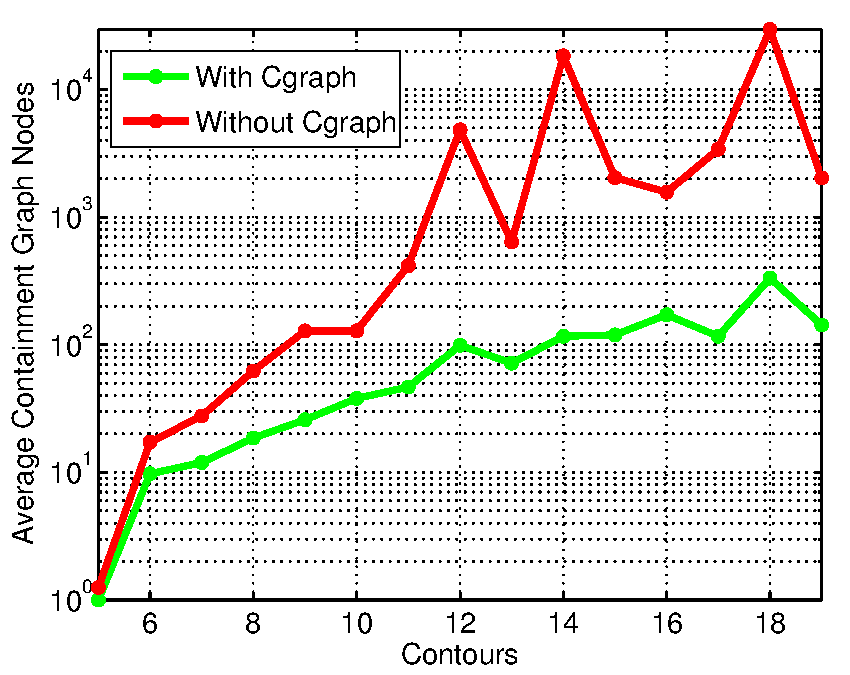
\includegraphics[width=0.43\linewidth]{figs/08_01_12_value_containment_graph.pdf}
  b)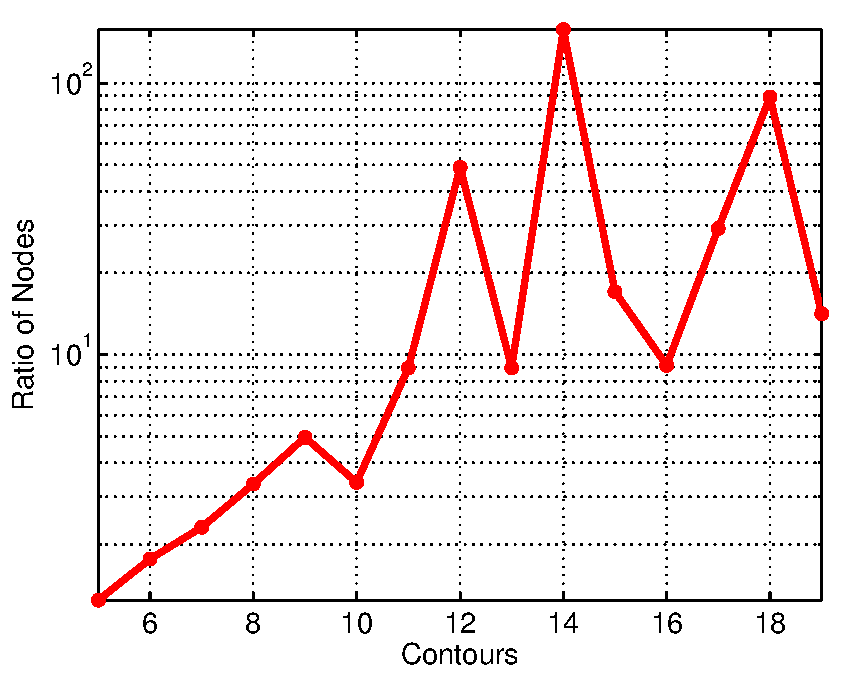
\includegraphics[width=0.43\linewidth]{figs/08_01_12_ratio.pdf}
 % %\vspace{-0.58cm}
  \caption{a) Average Number of Nodes with and without the containment graph versus the number of contours b) Ratio of Nodes with and without containment graph}
  \label{fig:graph_with_without}
  %\vspace{-0.65cm}
\end{figure}




 
% \begin{figure}[!h]
% \begin{center}
%  {\footnotesize\textit{(a)}} 
%   \includegraphics[width=0.43\linewidth]{figs/bag-of-fragments-1.png}
%  {\footnotesize\textit{(b)}} 
%   \includegraphics[width=0.43\linewidth]{figs/bag-of-fragments-2.png}
% \end{center}
% \begin{center} {\footnotesize\textit{(c)}}
%   \includegraphics[width=0.45\linewidth]{figs/bag-of-fragments-3.png}
%  {\footnotesize\textit{(d)}}\includegraphics[width=0.45\linewidth]{figs/bag-of-fragments-4.png}
% \end{center}  
% \begin{center} 
% {\footnotesize\textit{(e)}}
% \includegraphics[width=0.45\linewidth]{figs/bag-of-fragments-5.png}
%  {\footnotesize\textit{(f)}}
%  \includegraphics[width=0.45\linewidth]{figs/bag-of-fragments-6.png}
% \end{center}
% \caption{\FigureFont Can you recognize the object in the image from the
% fragment set above? Our approach has an abundant fragment representation, but this ensures that at least a few recognizable fragments are formed. Of 52 images that
% we ran, the subjects were able to tell the object category, \eg giraffe, or nearby category horse/donkey, in 50 cases. The two failure cases are shown in (e-f). (a-d)\ are prototypical
% cases.}
% \label{fig:bag:of:fragments}
% %\vspace{-0.5cm}
% \end{figure}





